% =============================================================
%  HAC-Net: Hybrid Attention-Based Convolutional Networks for
%  Protein-Ligand Binding Affinity
%  Series B: Deep Learning for Molecules, Post 1b
%  Compiles with pdfLaTeX on Overleaf (no extra files needed).
% =============================================================
\documentclass[11pt]{article}

\usepackage[margin=1in]{geometry}
\usepackage[T1]{fontenc}
\usepackage{lmodern}
\usepackage{microtype}
\usepackage{amsmath,amssymb,bm}
\usepackage{booktabs}
\usepackage{enumitem}
\usepackage{xcolor}
\usepackage{listings}
\usepackage{tikz}
\usetikzlibrary{arrows.meta,positioning,calc}
\usepackage{pgfplots}
\pgfplotsset{compat=1.16}
\usepackage[most]{tcolorbox}
\usepackage[colorlinks=true,linkcolor=blue!50!black,urlcolor=blue!50!black]{hyperref}

\setlength{\parskip}{0.55em}
\setlength{\parindent}{0pt}

% ---------- macros ----------
\newcommand{\R}{\mathbb{R}}
\newcommand{\E}{\mathbb{E}}
\newcommand{\pK}{\mathrm{p}K}
\DeclareMathOperator{\softmax}{softmax}
\DeclareMathOperator{\softsign}{softsign}
\DeclareMathOperator{\Var}{Var}
\DeclareMathOperator{\Cov}{Cov}

% ---------- Colab links: edit the primer line after you upload the notebook to GitHub ----------
\newcommand{\colaburlrepo}{https://colab.research.google.com/github/gregory-kyro/HAC-Net/blob/main/HACNet.ipynb}
\newcommand{\colaburlprimer}{https://colab.research.google.com/github/YOUR-USER/YOUR-REPO/blob/main/notebooks/B1b_hacnet_primer_colab.ipynb}
\newcommand{\colabbutton}[2]{%
  \href{#1}{\tcbox[on line,colback=orange!15,colframe=orange!70!black,boxrule=0.6pt,arc=3pt,
    left=4pt,right=4pt,top=1pt,bottom=1pt]{\small\textbf{$\blacktriangleright$ #2}}}}
\newcommand{\tryit}[1]{\par\vspace{0.3em}\noindent
  \fcolorbox{orange!70!black}{orange!8}{\parbox{\dimexpr\linewidth-2\fboxsep-2\fboxrule\relax}{%
  \small $\blacktriangleright$ \textbf{Run it.} #1}}\par\vspace{0.3em}}

% ---------- code listings ----------
\definecolor{codebg}{RGB}{246,246,248}
\definecolor{codecomment}{RGB}{90,110,90}
\definecolor{codekw}{RGB}{30,60,160}
\lstset{
  language=Python,
  basicstyle=\ttfamily\small,
  keywordstyle=\color{codekw}\bfseries,
  commentstyle=\color{codecomment}\itshape,
  backgroundcolor=\color{codebg},
  frame=single,
  rulecolor=\color{black!15},
  breaklines=true,
  columns=fullflexible,
  showstringspaces=false,
  xleftmargin=0.5em,
  xrightmargin=0.5em,
  aboveskip=0.8em,
  belowskip=0.8em
}

% ---------- boxes ----------
\tcbuselibrary{skins,breakable}
\newtcolorbox{keybox}[1][]{
  enhanced, breakable, colback=blue!4, colframe=blue!50!black,
  fonttitle=\bfseries, title={#1}, boxrule=0.6pt, arc=2pt
}
\newtcolorbox{mathbox}[1][]{
  enhanced, breakable, colback=black!3, colframe=black!45,
  fonttitle=\bfseries, title={#1}, boxrule=0.6pt, arc=2pt
}
\newtcolorbox{warnbox}[1][]{
  enhanced, breakable, colback=red!4, colframe=red!60!black,
  fonttitle=\bfseries, title={#1}, boxrule=0.6pt, arc=2pt
}
\newtcolorbox{hypbox}[1][]{
  enhanced, breakable, colback=yellow!8, colframe=yellow!50!black,
  fonttitle=\bfseries, title={#1}, boxrule=0.6pt, arc=2pt
}

% ---------- title ----------
\title{\textbf{HAC-Net: Predicting Protein--Ligand Binding Affinity}\\[0.2em]
       with Attention, a 3D Convolutional Network and Two Graph Networks}
\author{\textit{Series B: Deep Learning for Molecules --- Post 1b}}
\date{}

\begin{document}
\maketitle
\thispagestyle{empty}

\begin{center}
\small
About 40 minutes of reading, plus the notebooks.\\
\textbf{Prerequisites:} Post A2 (neural networks) and a first idea of convolutions and attention (Post B1, B5); Post B3 (graph convolutions) helps.\\[0.5em]
\textbf{Notebook 1, the authors' package and tutorial:} \texttt{HACNet.ipynb} in the HAC-Net repository (GPU and PDBbind data needed)\\
\textbf{Notebook 2, the primer:} \texttt{B1b\_hacnet\_primer\_colab.ipynb} (CPU only; NumPy and SciPy; rebuilds every building block)\\[0.4em]
\colabbutton{\colaburlrepo}{Open the authors' notebook}\quad
\colabbutton{\colaburlprimer}{Open the primer}\quad
{\footnotesize (see Section~\ref{sec:runit})}
\end{center}

\vspace{0.5em}
\hrule
\vspace{0.5em}

% =============================================================
\section{The question}
% =============================================================
A drug works by binding to a protein, and how tightly it binds is the \textbf{binding affinity}. Measuring affinity for every candidate molecule is slow and expensive, so a model that predicts affinity from the \emph{three-dimensional structure} of a protein--ligand complex would make it possible to screen enormous numbers of candidates computationally. It would also help to design proteins with desired binding properties.

\textbf{HAC-Net} (Hybrid Attention-Based Convolutional Neural Network; Kyro, Brent and Batista, \emph{J.\ Chem.\ Inf.\ Model.}\ \textbf{63}, 1947, 2023) combines three networks that look at the same complex in two different ways: a \textbf{3D convolutional network} that reads the complex as a voxel image, and two \textbf{graph convolutional networks} that read it as a graph of atoms. Attention appears in both: \emph{channel-wise} attention in the image branch and \emph{node-wise} attention in the graph branches. At the time of its publication, HAC-Net reported the lowest error among published models on the standard PDBbind v.2016 core-set benchmark.

This post introduces the model block by block, and then asks what its numbers do and do not show. The second part is where the paper's own tables turn out to be informative: from them we can extract, for example, the spread of the labels in each test set, and see how much a ligand-only or protein-only model already explains.

\begin{keybox}[Where the numbers come from, and what we could not do]
The architecture, training recipe and all results below are those of the paper (we read the arXiv version, with its published counterpart cited above). The code is the authors' open-source repository (MIT license), which contains the \texttt{HACNet} Python package (\texttt{pip install HACNet}) and a tutorial notebook. \textbf{We could not read the package's source code, run the authors' notebook, or access the PDBbind data here}, so the primer notebook is an \emph{independent reimplementation of each building block from the paper's description}, in NumPy, applied to a synthetic complex with random weights. It verifies mechanics (shapes, parameter counts, invariances, costs) and checks the paper's own statements against each other, but it does \textbf{not} train HAC-Net or reproduce its accuracy. Every accuracy number in this post is the paper's, not ours. Where the paper leaves a detail open, we say so.
\end{keybox}

% =============================================================
\section{Step 1: Affinity, units, and the data}
% =============================================================
Affinity is quoted as $\pK=-\log_{10}K$, where $K$ is a dissociation constant $K_D$ or an inhibition constant $K_i$ (in mol/L). A larger $\pK$ means tighter binding. The binding free energy is $\Delta G^\circ=-RT\ln10\cdot\pK$, so at $298.15$ K one $\pK$ unit is $\mathbf{1.364}$ \textbf{kcal/mol}, and an error of one $\pK$ unit is an error of a factor $10$ in $K$ (Supplement~\hyperref[sec:S1]{S1}). HAC-Net's headline error, RMSE $=1.205$ pK, is therefore $1.64$ kcal/mol, or a factor of $16$ in $K$. ``Chemical accuracy'' ($1$ kcal/mol) would be $0.733$ pK.

\textbf{The data} come from the PDBbind database: experimentally determined affinities for complexes deposited in the Protein Data Bank. The paper uses PDBbind v.2020: $19{,}443$ complexes, of which $5316$ form the \emph{refined set}, selected for high-quality structures and labels. Each entry gives the protein and the protein pocket (all residues within $10$ \AA\ of the ligand), the ligand structure, and the affinity as either $\pK_D$ or $\pK_I$ (the paper uses both and calls the predicted quantity $\pK_D$). The standard \textbf{test benchmark} is the \emph{PDBbind v.2016 core set}: $290$ complexes spanning a wide range of structural clusters and affinities. All HAC-Net results use training, validation and test sets with no overlap, and hyperparameters were chosen on training and validation data only.

\textbf{Preprocessing.} Hydrogens are added to each protein pocket with UCSF Chimera and the pocket is converted to MOL2; partial charges are computed with the Atomic Charge Calculator~II (an electronegativity equalization method). Four complexes could not be processed, and $34$ of $19{,}438$ ($0.17\%$) were dropped because some atom received an implausible charge of magnitude above $2$.

\textbf{Atom features.} Both branches describe each heavy atom with features from the earlier model Pafnucy: $9$ bits for the atom type (B, C, N, O, P, S, Se, halogen, metal), the hybridization ($1$, $2$ or $3$), the number of bonds to heavy atoms, the number of bonds to heteroatoms, $5$ bits (hydrophobic, aromatic, acceptor, donor, ring), the partial charge, and $+1$ or $-1$ for ligand or protein. That is $9+1+1+1+5+1+1=\mathbf{19}$ numbers. The graph branches add the van der Waals radius, for $\mathbf{20}$ features.

\tryit{Primer \S1--2. Convert $\pK$ to kcal/mol, and build a synthetic complex with the $19$ and $20$ features.}

% =============================================================
\section{Step 2: One complex, two views}
% =============================================================
The same complex is presented twice (Figure~\ref{fig:overview}).

\begin{figure}[ht]
\centering
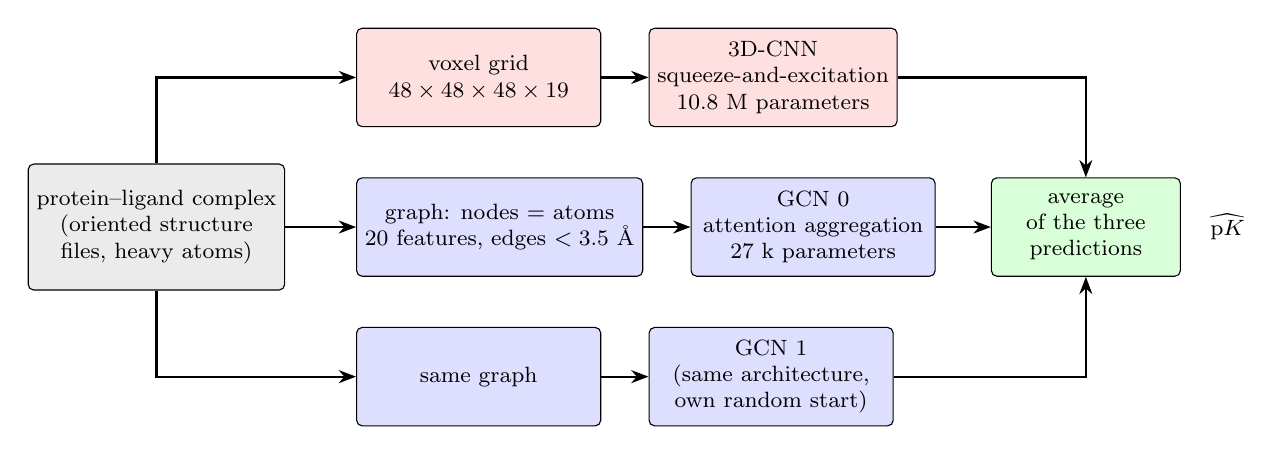
\begin{tikzpicture}[
  box/.style={draw, rounded corners=2pt, minimum height=1.25cm, minimum width=3.1cm, align=center, font=\footnotesize, inner sep=3pt},
  gray/.style={box, fill=black!8},
  cn/.style={box, fill=red!12},
  gc/.style={box, fill=blue!13},
  av/.style={box, fill=green!15},
  arr/.style={-{Stealth[length=2.2mm]}, thick}
]
\node[gray, minimum height=1.6cm] (cx) {protein--ligand complex\\(oriented structure\\files, heavy atoms)};
\node[cn, right=0.9cm of cx, yshift=1.9cm] (vox) {voxel grid\\$48\times48\times48\times19$};
\node[cn, right=0.6cm of vox] (cnn) {3D-CNN\\squeeze-and-excitation\\10.8 M parameters};
\node[gc, right=0.9cm of cx] (gr) {graph: nodes $=$ atoms\\20 features, edges $<3.5$ \AA};
\node[gc, right=0.6cm of gr, yshift=0.0cm] (g0) {GCN 0\\attention aggregation\\27 k parameters};
\node[gc, right=0.9cm of cx, yshift=-1.9cm] (gr2) {same graph};
\node[gc, right=0.6cm of gr2] (g1) {GCN 1\\(same architecture,\\own random start)};
\node[av, right=0.7cm of g0, yshift=-0.0cm, minimum width=2.4cm] (avg) {average\\of the three\\predictions};
\draw[arr] (cx.north) |- (vox.west); \draw[arr] (cx) -- (gr); \draw[arr] (cx.south) |- (gr2.west);
\draw[arr] (vox) -- (cnn); \draw[arr] (gr) -- (g0); \draw[arr] (gr2) -- (g1);
\draw[arr] (cnn.east) -| (avg.north); \draw[arr] (g0) -- (avg); \draw[arr] (g1.east) -| (avg.south);
\node[right=0.25cm of avg, font=\footnotesize] {$\widehat{\pK}$};
\end{tikzpicture}
\caption{HAC-Net. The complex is voxelized for the 3D-CNN (red) and turned into a graph for two identical graph networks (blue); the three predicted $\pK$ values are averaged. The graph branches use only distances between atoms; the voxel grid depends on how the complex is oriented in space.}
\label{fig:overview}
\end{figure}

\textbf{As an image (voxel grid).} Each heavy atom is placed in a $48\times48\times48$ grid of $1$ \AA\ voxels centered on the complex, and the voxel holds the atom's $19$ features (empty voxels hold zeros). In PDBbind, $0.22\%$ of atoms share a voxel with another atom (their features are summed) and $0.01\%$ fall outside the grid and are omitted. The grid is a four-dimensional array with $48^3\times19=2{,}101{,}248$ numbers, mostly zeros: in our synthetic complex of $878$ atoms only $0.79\%$ of the voxels are occupied.

\textbf{As a graph.} Nodes are the heavy atoms with $20$ features each, and two atoms are joined by an edge if their centers are within $3.5$ \AA. In the synthetic complex this gives $9712$ directed edges, a mean of $11.1$ neighbors per atom. The graph needs no orientation: it only uses interatomic distances.

\tryit{Primer \S2. Voxelize and build the graph for the synthetic complex; compare the sizes of the two representations.}

% =============================================================
\section{Step 3: The 3D convolutional network}
% =============================================================
\subsection*{Convolution on a voxel grid}
A 3D convolutional layer slides a learned filter over the grid. For a filter of side $k$ with $F$ input channels (here the feature dimensions) and output channel $c$, stride $s$ and padding $p$ (Eq.~1 of the paper),
\[
  \text{out}[x',y',z',c]=b_c+\sum_{h,i,j=1}^{k}\sum_{f=1}^{F}\text{filter}[h,i,j,f,c]\;\text{in}[sx'+h-p,\ sy'+i-p,\ sz'+j-p,\ f],
\]
with output side length $\lfloor(n+2p-k)/s\rfloor+1$. Many filters give many output channels. A convolution has $k^3FC+C$ parameters, independent of the grid size.

Because the grid is nearly empty, the \emph{first} convolution has a cheap alternative: it is linear, so its output is the sum, over atoms, of a copy of the filter weighted by the atom's features ("atom stamps"). The primer implements the convolution three ways (direct loops, one matrix product on unfolded patches, and atom stamping) and the three agree to $10^{-15}$ (Supplement~\hyperref[sec:S2]{S2}).

\subsection*{The squeeze-and-excitation block}
The key attention component of the 3D-CNN is the \textbf{squeeze-and-excitation (SE) block} of Hu et al.\ (the 2017 ImageNet classification winner). After a convolution produces a feature map $\mathbf u$ with $F$ channels:
\begin{enumerate}[nosep]
  \item \textbf{Squeeze:} average each channel over all positions, $z_c=\frac1{L^3}\sum_{ijk}u[i,j,k,c]$, giving a vector $\mathbf z\in\R^F$.
  \item \textbf{Excite:} $\mathbf s=\sigma\big(\mathrm{ReLU}(\mathbf zW_1)W_2\big)$ with $W_1\in\R^{F\times F/16}$, $W_2\in\R^{F/16\times F}$, so every $s_c\in(0,1)$.
  \item \textbf{Scale:} $x[i,j,k,c]=s_c\,u[i,j,k,c]$.
\end{enumerate}
The model thus learns to weight its channels by a function of their \emph{overall} activity in this particular complex: channel-wise self-attention (Supplement~\hyperref[sec:S3]{S3}). In the primer, the channel weights for a $64$-channel map lie in $(0.15,\,0.87)$ and differ from one input to another. The two small fully connected layers of the three SE blocks add only $11{,}228$ parameters, $0.1\%$ of the network.

\subsection*{The architecture}
\begin{figure}[ht]
\centering
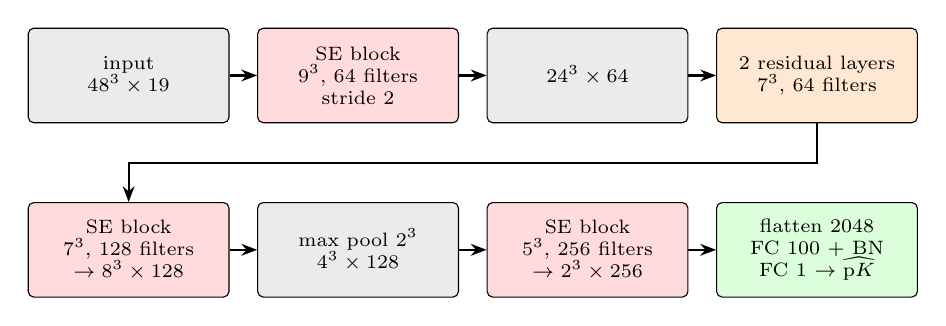
\begin{tikzpicture}[
  box/.style={draw, rounded corners=2pt, minimum height=1.2cm, minimum width=2.55cm, align=center, font=\scriptsize, inner sep=2pt},
  dat/.style={box, fill=black!8},
  se/.style={box, fill=red!14},
  rs/.style={box, fill=orange!18},
  fc/.style={box, fill=green!14},
  arr/.style={-{Stealth[length=2mm]}, thick}
]
\node[dat] (a) {input\\$48^3\times19$};
\node[se, right=0.35cm of a] (b) {SE block\\$9^3$, 64 filters\\stride 2};
\node[dat, right=0.35cm of b] (c) {$24^3\times64$};
\node[rs, right=0.35cm of c] (d) {2 residual layers\\$7^3$, 64 filters};
\draw[arr] (a)--(b); \draw[arr] (b)--(c); \draw[arr] (c)--(d);
\node[se, below=1.0cm of a] (e) {SE block\\$7^3$, 128 filters\\$\to8^3\times128$};
\node[dat, right=0.35cm of e] (f) {max pool $2^3$\\$4^3\times128$};
\node[se, right=0.35cm of f] (g) {SE block\\$5^3$, 256 filters\\$\to2^3\times256$};
\node[fc, right=0.35cm of g] (h) {flatten 2048\\FC 100 + BN\\FC 1 $\to\widehat{\pK}$};
\draw[arr] (d.south) -- ++(0,-0.5) -| (e.north); \draw[arr] (e)--(f); \draw[arr] (f)--(g); \draw[arr] (g)--(h);
\end{tikzpicture}
\caption{The 3D-CNN. Every convolution is followed by ReLU and batch normalization. The sizes are those given in the paper; the strides and paddings, which the paper does not give, are determined by them up to the choices listed in the text.}
\label{fig:cnn}
\end{figure}

The layers, from the paper: the input $48\times48\times48\times19$ goes through an SE block with $9\times9\times9$ filters and $64$ channels (to $24^3\times64$); two residual layers of $7\times7\times7$ filters with $64$ channels (a residual layer adds a skip connection around a convolution); an SE block with $7^3$ filters and $128$ channels (to $8^3\times128$); a $2\times2\times2$ max pool ($4^3\times128$); an SE block with $5^3$ filters and $256$ channels ($2^3\times256$); and finally the $2048$ numbers are flattened and passed through fully connected layers $2048\to100\to1$ to give the predicted $\pK$.

\textbf{What the paper leaves open.} It does not state strides or paddings. The stated sizes pin them down quite far (primer \S3): the first block must use stride $2$ and padding $4$; the residual layers stride $1$ and padding $3$; the second SE block stride $3$ with padding $2$ or $3$; and the third has several options (stride $1$ with padding $1$, or stride $2$ with padding $2$, among others).

\subsection*{Parameters and cost, and a check of the paper}
The paper states that the fully connected layers hold $1.9\%$ of the 3D-CNN's parameters, and this statement resolves an ambiguity in the description. Counting parameters from the stated architecture (convolution weights and biases, batch-norm scale and shift, SE layers, fully connected layers):

\begin{center}
\small
\begin{tabular}{@{}lrrrr@{}}
\toprule
Stage & Parameters & \% & Multiply-adds & \% of compute\\
\midrule
SE block 1 ($9^3\times19@64$) & $887{,}236$ & $8.2$ & $1.23\times10^{10}$ & $23.3$\\
Two residual layers ($7^3\times64@64$) & $2{,}810{,}240$ & $26.0$ & $3.88\times10^{10}$ & $73.9$\\
SE block 2 ($7^3\times64@128$) & $2{,}812{,}424$ & $26.0$ & $1.44\times10^{9}$ & $2.7$\\
SE block 3 ($5^3\times128@256$) & $4{,}105{,}232$ & $37.9$ & $3.3\times10^{7}$ & $0.06$\\
Fully connected $2048\to100\to1$ & $205{,}201$ & $1.9$ & $2\times10^{5}$ & $0.0$\\
\midrule
Total & $10{,}820{,}333$ & $100$ & $5.26\times10^{10}$ & $100$\\
\bottomrule
\end{tabular}
\end{center}

If each ``residual layer'' is \emph{one} convolution with a skip connection, the fully connected share is $\mathbf{1.90\%}$, exactly the paper's number. If each residual layer contained two convolutions, the network would have $13.6$ million parameters and the share would be $1.51\%$. So the first reading is the right one.

\begin{figure}[ht]
\centering
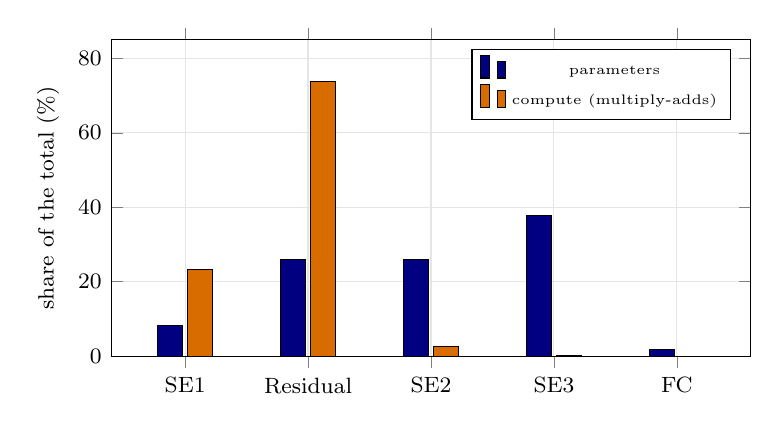
\begin{tikzpicture}
\begin{axis}[ybar, width=0.8\textwidth, height=5.6cm, bar width=9pt, symbolic x coords={SE1, Residual, SE2, SE3, FC}, xtick=data,
  ylabel={share of the total (\%)}, ymin=0, ymax=85, grid=major, grid style={black!10}, legend pos=north east, legend style={font=\tiny},
  tick label style={font=\footnotesize}, label style={font=\footnotesize}, enlarge x limits=0.15]
\addplot[fill=blue!50!black] coordinates {(SE1,8.2) (Residual,26.0) (SE2,26.0) (SE3,37.9) (FC,1.9)};
\addplot[fill=orange!85!black] coordinates {(SE1,23.3) (Residual,73.9) (SE2,2.7) (SE3,0.06) (FC,0)};
\legend{parameters, compute (multiply-adds)}
\end{axis}
\end{tikzpicture}
\caption{Where the parameters and where the compute of the 3D-CNN live. The parameters sit in the late, low-resolution layers; the compute sits in the early, high-resolution ones ($24^3$ positions), above all the two residual layers.}
\label{fig:cost}
\end{figure}

Two practical consequences. One complex costs about $5\times10^{10}$ multiply-adds in the 3D-CNN, independent of how many atoms it has. And the voxel grid alone takes $8.4$ MB in float32 and the first feature map $3.5$ MB per complex; in the paper the 3D-CNN is trained with batches of $50$ complexes (the graph networks with batches of $7$).

\subsection*{Training: two stages}
The 3D-CNN is trained for $100$ epochs with batch size $50$, mean squared error loss and the RMSProp optimizer (initial learning rate $7\times10^{-4}$). After each epoch it is evaluated on the validation set, and the checkpoint with the highest average of Spearman $\rho$ and Pearson $r$ is kept. A second stage then extracts the $2048$-dimensional flattened features and trains a fresh pair of fully connected layers on them (with batch-norm momentum $0.3$ instead of $0.1$), selecting a checkpoint in the same way. The authors motivate this by the fact that the fully connected layers hold so few of the parameters ($1.9\%$) that the first stage is driven by the convolutional ones.

\tryit{Primer \S3--5. Three implementations of the 3D convolution, the SE block, and the parameter and compute table above, including the $1.90\%$ check.}

% =============================================================
\section{Step 4: The graph convolutional networks}
% =============================================================
Each graph network (Figure~\ref{fig:gcn}) iterates \textbf{message passing} four times and then forms one vector for the whole complex.

\begin{figure}[ht]
\centering
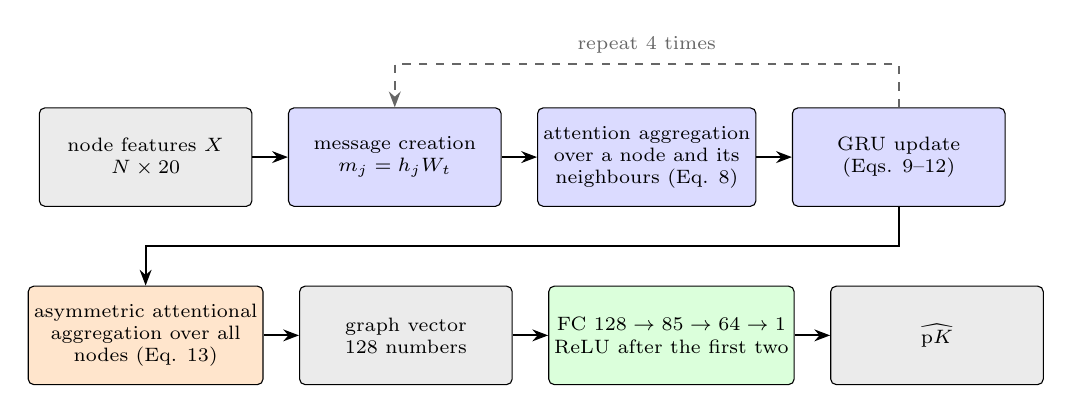
\begin{tikzpicture}[
  box/.style={draw, rounded corners=2pt, minimum height=1.25cm, minimum width=2.7cm, align=center, font=\scriptsize, inner sep=2pt},
  dat/.style={box, fill=black!8},
  mp/.style={box, fill=blue!14},
  ag/.style={box, fill=orange!20},
  fc/.style={box, fill=green!14},
  arr/.style={-{Stealth[length=2mm]}, thick}
]
\node[dat] (x) {node features $X$\\$N\times20$};
\node[mp, right=0.45cm of x] (m) {message creation\\$m_j=h_jW_t$};
\node[mp, right=0.45cm of m] (a) {attention aggregation\\over a node and its\\neighbours (Eq. 8)};
\node[mp, right=0.45cm of a] (g) {GRU update\\(Eqs. 9--12)};
\draw[arr] (x)--(m); \draw[arr] (m)--(a); \draw[arr] (a)--(g);
\draw[arr, dashed, black!60] (g.north) -- ++(0,0.55) -| node[above, pos=0.25, font=\scriptsize] {repeat 4 times} (m.north);
\node[ag, below=1.0cm of x] (s) {asymmetric attentional\\aggregation over all\\nodes (Eq. 13)};
\node[dat, right=0.45cm of s] (v) {graph vector\\128 numbers};
\node[fc, right=0.45cm of v] (f) {FC $128\to85\to64\to1$\\ReLU after the first two};
\node[dat, right=0.45cm of f] (o) {$\widehat{\pK}$};
\draw[arr] (g.south) -- ++(0,-0.5) -| (s.north); \draw[arr] (s)--(v); \draw[arr] (v)--(f); \draw[arr] (f)--(o);
\end{tikzpicture}
\caption{One graph network of HAC-Net. The two GCNs are identical in architecture and differ only in their random initialization and training.}
\label{fig:gcn}
\end{figure}

\textbf{Message creation.} A linear map that preserves the dimension (20) turns each atom's features into a message.

\textbf{Attention aggregation (Eq.~8).} For each atom $i$, consider the set $S_i$ consisting of $i$ and its neighbors. A small network $\Gamma$ (fully connected layers $20\to10\to5\to1$ with softsign activation after the first two) gives each message a score, a softmax over $S_i$ turns the scores into weights $\alpha_{ij}$, and the aggregate is $\sum_{j\in S_i}\alpha_{ij}\,m_j$. The paper adds that the neighbors' messages are weighted by their \emph{distance} from the central atom. The weights $\alpha_{ij}$ are positive and sum to $1$, so the result is a weighted average whose size does not grow with the number of neighbors.

\textbf{Update (Eqs.~9--12).} A gated recurrent unit (GRU) combines the atom's previous features $h$ with the aggregate $x$ through a reset gate $r$, an update gate $z$ and a candidate $n$:
\[
  r=\sigma(W_{xr}x+W_{hr}h),\quad z=\sigma(W_{xz}x+W_{hz}h),\quad n=\tanh\big(W_{xn}x+r\odot W_{hn}h\big),\quad y=(1-z)\odot n+z\odot h .
\]
After four rounds each atom has seen the atoms within four edges ($\le4\times3.5$ \AA).

\textbf{Asymmetric attentional aggregation (Eq.~13).} To get one vector for the complex, a gate network $\Gamma$ ($40\to20\to128$) looks at the \emph{concatenation} of each atom's final features $Y_v$ and its \emph{original} features $X_v$, and a softmax over \textbf{all atoms} (separately for each of $128$ channels) gives the weights; they multiply $\Omega X_v$ ($20\to128$, from the original features only) and are summed over atoms. This is the ``asymmetric'' readout of Jones et al.\ (the FAST model). Three fully connected layers ($128\to85\to64\to1$) produce the prediction.

\textbf{Parameters.} In our implementation (four separate message matrices, as in the usual gated graph convolution, and no bias on them) the branch has $\mathbf{27{,}121}$ parameters, of which $16{,}534$ ($61.0\%$) are in the final fully connected layers. The paper states $59.5\%$; we cannot account for the difference of about $590$ parameters from the text, which suggests a small component that the paper does not describe.

\textbf{What the paper leaves open.} Exactly how messages are ``weighted by the distance'' (we use the literal reading, multiplying by $d_{ij}$, and $1$ for the central atom); whether the message matrices are separate per round (we assume so); and the exact input scaling. These affect numbers but not the structure; the primer lets you change the weighting (Exercise~4).

\subsection*{Properties we can test without data}
On the synthetic complex with random weights: the attention weights of every neighborhood sum to $1$; relabeling the atoms at random changes the output by $4\times10^{-15}$ (the graph branch cannot depend on atom order); and rotating the whole complex also changes it by $4\times10^{-15}$ (it uses only distances). For the 3D-CNN the same rotation changes which voxels are occupied: the voxel grid is \textbf{not} rotation invariant, and the paper describes the inputs as \emph{oriented} structure files and does not describe rotation augmentation.

For the cost, the graph branch needs about $2.7\times10^{7}$ multiply-adds for the $878$-atom complex, roughly $2000$ times fewer than the 3D-CNN; but it grows with the number of atoms and edges, while the 3D-CNN's cost is fixed.

\subsection*{Why attention in the readout? A small trained demonstration}
The paper compares HAC-Net with a ``vanilla'' version without the attention components and reports that attention improves its performance significantly (the numbers are shown only in a figure). We cannot retrain HAC-Net, but we can isolate the mechanism in a toy where the answer is known. A ``complex'' is a set of $20$ to $60$ nodes, each with a marker $m_v\in\{0,1\}$ (about $15\%$ are marked, like atoms at the binding interface), a signal $s_v$ and a noise feature. The label is the \emph{average signal of the marked nodes only}. We fit three readouts by least squares:

\begin{center}
\small
\begin{tabular}{@{}lcc@{}}
\toprule
Readout & Test RMSE & Test $R^2$\\
\midrule
Baseline (predict the mean) & $0.443$ & $0$\\
Sum: $\sum_vw\cdot x_v$ & $0.419$ & $0.11$\\
Mean: $\frac1N\sum_vw\cdot x_v$ & $0.411$ & $0.14$\\
Attention: $\sum_v\softmax_v(\gamma\cdot x_v)\,(\omega\cdot x_v)$ & $\mathbf{0.096}$ & $\mathbf{0.95}$\\
\bottomrule
\end{tabular}
\end{center}

A linear readout followed by a sum or a mean can only depend on the \emph{totals} of the features, so it cannot compute ``signal times marker''; the attention readout can, and it learns to put $99.6\%$ of its weight on the marked nodes (which are $15.4\%$ of all nodes) (Supplement~\hyperref[sec:S4]{S4}). This is a toy: it shows why a learned, input-dependent weighting is more expressive than a plain sum, not how much it helps on real complexes.

\tryit{Primer \S6 and \S9. Run the graph forward pass, the invariance tests, the cost count, and the three readouts.}

% =============================================================
\section{Step 5: The hybrid, and its training}
% =============================================================
The final prediction averages the outputs of the three networks. (We read ``averages the outputs'' as a plain mean of three predictions, so the pair of GCNs carries two thirds of the weight; the paper does not state the weights.) The authors describe the two GCNs as the stronger components, the 3D-CNN as complementary because it learns in a different way, and the second GCN as a way of damping the noise of stochastic training.

That last point has a simple quantitative form. If two predictors have errors of equal variance $\sigma^2$ and correlation $\rho$, their mean has variance $\sigma^2(1+\rho)/2$ (for $n$ predictors, $\sigma^2[1+(n-1)\rho]/n$; Supplement~\hyperref[sec:S7]{S7}):

\begin{center}
\small
\begin{tabular}{@{}lccc@{}}
\toprule
Error correlation $\rho$ & $0$ & $0.5$ & $0.8$\\
\midrule
Error std of the mean of two, relative to one & $0.707$ & $0.866$ & $0.949$\\
\bottomrule
\end{tabular}
\end{center}

Averaging helps in proportion to how \emph{different} the errors are, which is why two GCNs trained from different random starts help, and why a differently built 3D-CNN is a useful third member.

\textbf{GCN training.} Each GCN is trained for $300$ epochs with batch size $7$, mean squared error, Adam with a constant learning rate of $0.001$, and the checkpoint with the highest average of Spearman $\rho$ and Pearson $r$ on the validation set is kept. Validation and test sets are constructed to contain equal numbers of complexes from each percentile of the affinity distribution, so that performance is assessed across the whole affinity range.

% =============================================================
\section{Step 6: Results}
% =============================================================
On the PDBbind v.2016 core set (selected rows of the paper's Table~1; the full table has $24$ models):

\begin{center}
\small
\begin{tabular}{@{}lccccc@{}}
\toprule
Model & RMSE & MAE & $R^2$ & Pearson $r$ & Spearman $\rho$\\
\midrule
\textbf{HAC-Net} & $\mathbf{1.205}$ & $0.971$ & $0.692$ & $0.846$ & $0.843$\\
AEScore & $1.22$ & --- & --- & $0.83$ & $0.64$\\
DeepAtom & $1.232$ & $0.904$ & --- & $0.831$ & ---\\
HAC-Net, trained on the v.2016 refined set & $1.259$ & $1.020$ & $0.664$ & $0.819$ & $0.814$\\
FAST & $1.308$ & $1.019$ & $0.638$ & $0.810$ & $0.807$\\
Pafnucy & $1.42$ & $1.13$ & --- & $0.78$ & ---\\
\bottomrule
\end{tabular}
\end{center}

The best HAC-Net is trained on all complexes of the v.2020 general set that are not in the core set or in its random validation set; the other models were trained on a variety of other sets (some on the smaller v.2016 refined set, which can be better matched to the core set). The authors flag this as one reason why such a table cannot settle every question, and motivate the generalization tests below. Models marked with an asterisk in the full table did not use a validation set, which the authors expect to give optimistic results.

\textbf{What the numbers mean.} RMSE $1.205$ pK is $1.64$ kcal/mol; MAE $0.971$ pK is $1.33$ kcal/mol. Beyond scoring, the paper also runs the CASF-2016 ranking, docking and screening tests: a ranking Spearman $\rho$ of $0.705$, docking success rates of $0.368$, $0.572$, $0.702$ for the top 1, 2 and 3 poses, and screening success rates of identifying the best binder in the top $1\%$, $5\%$, $10\%$ of $0.088$, $0.211$, $0.386$ (forward screening). The authors state that HAC-Net does not match docking programs such as AutoDock Vina on these tasks, which is unsurprising since it is not trained for them, and propose combining the two kinds of method.

\subsection*{What label spread do the tables imply?}
The coefficient of determination is $R^2=1-\mathrm{MSE}/\Var(y)$, so every row with an RMSE and an $R^2$ implies the standard deviation of the labels of its test set, $\sigma=\mathrm{RMSE}/\sqrt{1-R^2}$. For the three core-set rows above this gives $\sigma=2.171,\ 2.172,\ 2.174$ pK: the three models were tested on the same set, and the three implied spreads agree to $0.003$. So the core set has a label standard deviation of about $\mathbf{2.17}$ \textbf{pK}; a model that always predicted the mean label would have an RMSE of about $2.17$, and HAC-Net's $1.205$ is $55\%$ of that. This simple calculation is a useful sanity check on any published table, and we will use it below. It also shows that $R^2\le r^2$ in every row ($0.692\le0.716$ for HAC-Net): the difference measures how well the predictions are calibrated, not only correlated.

\tryit{Primer \S8. Recompute the implied spreads from the table rows.}

% =============================================================
\section{Step 7: Does it generalize?}
% =============================================================
The authors take a central concern of the field seriously: deep models for binding affinity may perform well mainly because test complexes resemble training complexes. They test HAC-Net on splits that maximize the difference between training and test sets in several ways, with the following results:

\begin{center}
\small
\begin{tabular}{@{}lcccc@{}}
\toprule
Test set & RMSE & $R^2$ & Pearson $r$ & Implied $\sigma$ (pK)\\
\midrule
v.2007 core set (control) & $1.447$ & $0.598$ & $0.807$ & $2.28$\\
Protein-structure split (TM-score clusters) & $1.472$ & $0.608$ & $0.799$ & $2.35$\\
Protein-sequence split (identity clusters) & $1.301$ & $0.583$ & $0.796$ & $2.02$\\
Ligand split (ECFP4, Tanimoto $0.8$) & $1.240$ & $0.355$ & $0.597$ & $1.54$\\
10-fold CV, ligand dissimilarity: control (v.2016 core) & $1.432$ & $0.567$ & $0.761$ & $2.18$\\
10-fold CV, mean of 10 test sets & $1.473$ & $0.430$ & $0.665$ & $1.95$\\
\bottomrule
\end{tabular}
\end{center}

The protein-based splits barely change anything: the model's accuracy does not depend much on seeing similar protein structures or sequences. The ligand-based splits reduce the correlations considerably (to $r=0.60$ and $0.67$) while the RMSE changes little, and the paper attributes this to training with a mean-squared-error loss.

\begin{figure}[ht]
\centering
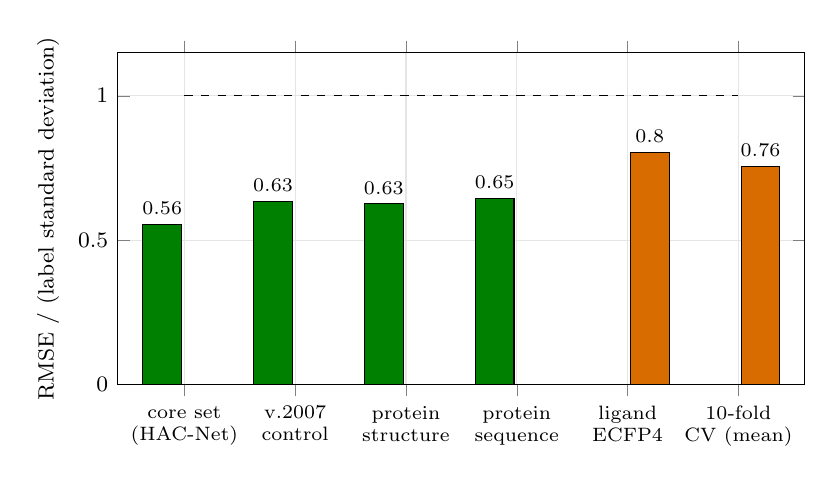
\begin{tikzpicture}
\begin{axis}[ybar, width=0.85\textwidth, height=5.8cm, bar width=14pt, symbolic x coords={Core, Control07, Structure, Sequence, Ligand, CV10}, xtick={Core, Control07, Structure, Sequence, Ligand, CV10},
  xticklabels={core set\\(HAC-Net), v.2007\\control, protein\\structure, protein\\sequence, ligand\\ECFP4, 10-fold\\CV (mean)},
  x tick label style={font=\scriptsize, align=center}, ylabel={RMSE / (label standard deviation)}, ymin=0, ymax=1.15, grid=major, grid style={black!10},
  tick label style={font=\footnotesize}, label style={font=\footnotesize}, enlarge x limits=0.12, nodes near coords, nodes near coords style={font=\scriptsize}, every node near coord/.append style={/pgf/number format/fixed, /pgf/number format/precision=2}]
\addplot[fill=green!50!black] coordinates {(Core,0.555) (Control07,0.634) (Structure,0.626) (Sequence,0.646)};
\addplot[fill=orange!85!black] coordinates {(Ligand,0.803) (CV10,0.755)};
\draw[black, dashed] (axis cs:Core,1) -- (axis cs:CV10,1);
\end{axis}
\end{tikzpicture}
\caption{Error relative to the spread of the labels in each test set, $\mathrm{RMSE}/\sigma$ with $\sigma$ implied by RMSE and $R^2$. A model that always predicts the mean label has $\mathrm{RMSE}/\sigma=1$ (dashed). The ligand-based splits (orange) are the hardest relative to their label spread.}
\label{fig:rel}
\end{figure}

\textbf{A complementary reading.} The column of implied spreads shows that the ligand splits have a \emph{narrower} label distribution ($\sigma=1.54$ and $1.95$ pK) than the core sets ($2.17$ to $2.35$). RMSE is not comparable across test sets with different spreads: the same $1.24$ pK is $55\%$ of the spread on the core set and $80\%$ of it on the ligand split (Figure~\ref{fig:rel}). So part of the reason why the RMSE changes little while the correlations fall is that the test sets are narrower, and in relative terms the error does grow, from $0.56$--$0.66$ to $0.76$--$0.80$ of the spread. This is consistent with the paper's main message, that ligand dissimilarity hurts more than protein dissimilarity, and it adds one more way of seeing it.

\begin{sloppypar}
\textbf{Cross-validation consistency.} The ten cross-validation test sets have implied spreads between $1.94$ and $1.96$ pK, as expected from the way the test sets were built (equal numbers from each affinity percentile). From the ten rows of the paper's Table~3 we recompute the means ($1.473,\ 1.170,\ 0.430,\ 0.664,\ 0.670$) and standard deviations ($0.029,\ 0.024,\ 0.023,\ 0.014,\ 0.014$), which agree with the paper's up to one unit in the last digit, and an average coefficient of variation of $0.027$ against the stated $0.026$. The runs are very reproducible, which supports the authors' claim that retrained versions meet the same standard. The cross-validation control (trained on about $3100$ complexes, roughly six times fewer than the main model) scores worse than the main result: $R^2=0.567$ against $0.692$.
\end{sloppypar}

\textbf{Lower-quality data.} On a test set of $1000$ complexes from the general set (about $75\%$ of which are not in the refined set), the paper finds a drop in correlation with a small change in error, and no relationship between crystal resolution and absolute error. It concludes that HAC-Net is not specialized to high-quality structures. (The numbers for this test are given only in a figure.)

\tryit{Primer \S8. Recompute the implied spreads and the cross-validation statistics.}

% =============================================================
\section{Step 8: Reading the evidence critically}
% =============================================================
\begin{enumerate}[nosep]
  \item \textbf{Memorization.} Following concerns raised by Volkov et al., the authors train and test HAC-Net with \emph{only the protein} or \emph{only the ligand}. On the core set the RMSE rises from $1.205$ to $1.742$ (protein only) and $1.605$ (ligand only), and the Pearson $r$ falls from $0.846$ to $0.638$ and $0.741$. With the spread of $2.17$, these RMSEs correspond to $R^2=0.36$ and $0.45$, against $0.69$ for the complex: \textbf{the protein alone already explains about half ($52\%$), and the ligand alone about two thirds ($66\%$), of what the whole complex explains}. The authors acknowledge that ``there is clearly a degree of memorization'' while noting that the complex does significantly better. For a user: a prediction for a ligand or a protein family far from the training data should be trusted much less than the benchmark suggests.
  \item \textbf{Comparisons across papers are fragile.} The models in Table~1 were trained on different data (Step~6), some without validation sets. The test set is the same, so the implied spread checks out (it is $2.17$ for three different models), but the training sets are not.
  \item \textbf{RMSE is not enough.} As in Step~7, compare errors with the spread of the labels, and use correlation metrics too. Neither alone tells whether a model has learned the physics.
  \item \textbf{The label is a mixture.} The target pools $\pK_D$ and $\pK_I$ values measured in different laboratories with different methods; part of the error is irreducible label noise (we cannot estimate it from the paper).
  \item \textbf{Orientation.} The voxel branch depends on the orientation of the input, which the paper states is aligned; the graph branches do not.
  \item \textbf{Time.} The paper's comparison reflects the literature at its writing (2022--2023). We have not surveyed more recent models.
\end{enumerate}

% =============================================================
\section{Run it yourself}
\label{sec:runit}
% =============================================================
\begin{keybox}[Which notebook?]
\begin{description}[leftmargin=0pt, nosep, labelindent=0pt]
  \item[Primer] \colabbutton{\colaburlprimer}{Open the primer}\ \ \texttt{B1b\_hacnet\_primer\_colab.ipynb}. CPU only, a few seconds, NumPy and SciPy, nothing to download. It rebuilds the building blocks and checks them; it \emph{does not train the model}. Start here.
  \item[The authors' package and tutorial] \colabbutton{\colaburlrepo}{Open the authors' notebook}\ \ In the repository \texttt{gregory-kyro/HAC-Net} (MIT license): install the package with \texttt{pip install HACNet} and use the tutorial notebook \texttt{HACNet.ipynb}. The repository links the training, validation and test sets (HDF files), the extracted 3D-CNN features, and trained model parameters. We have not run it; you need a GPU runtime and the data files.
\end{description}
\end{keybox}

\subsection{Where each step lives in the primer}
\begin{center}
\small
\begin{tabular}{@{}llp{6.4cm}@{}}
\toprule
Post & Primer & What you should see\\
\midrule
Step 1 & \S1--2 & $1$ pK $=1.364$ kcal/mol; $19$ and $20$ features\\
Step 2 & \S2 & $48^3\times19$ grid, $0.79\%$ occupied; $9712$ edges, mean degree $11.1$\\
Step 3 & \S3--5 & 3 convolutions agree; $10{,}820{,}333$ parameters, fully connected share $1.90\%$\\
Step 4 & \S6, \S9 & $27{,}121$ parameters; invariances to $10^{-15}$; attention RMSE $0.096$\\
Step 5 & \S7 & $0.707$, $0.866$, $0.949$ for $\rho=0,0.5,0.8$\\
Steps 6--8 & \S8 & implied label spread $2.17$; protein-only $52\%$, ligand-only $66\%$\\
\bottomrule
\end{tabular}
\end{center}

\subsection{The key calculations in one cell}
This script uses only the Python standard library and reproduces the unit conversion, the parameter count and the $1.90\%$ check, the implied label spreads, and the averaging factor:

\begin{lstlisting}
import math

# 1) units: pK <-> kcal/mol
kcal_per_pk = 0.0019872041 * 298.15 * math.log(10)
print(f"1 pK = {kcal_per_pk:.4f} kcal/mol; HAC-Net RMSE 1.205 pK = {1.205 * kcal_per_pk:.2f} kcal/mol")

# 2) parameters of the 3D-CNN of the paper (each residual layer = one convolution with a skip connection)
conv = lambda k, cin, cout: k**3 * cin * cout + cout
bn = lambda c: 2 * c
se = lambda F: 2 * F * (F // 16) + F // 16 + F                  # the two FC layers of a squeeze-and-excitation block
fc = 2048 * 100 + 100 + bn(100) + 101                            # 2048 -> 100 -> 1
total = (conv(9, 19, 64) + bn(64) + se(64) + 2 * (conv(7, 64, 64) + bn(64))
         + conv(7, 64, 128) + bn(128) + se(128) + conv(5, 128, 256) + bn(256) + se(256) + fc)
print(f"3D-CNN: {total:,} parameters; fully connected share {100 * fc / total:.2f} % (the paper says 1.9 %)")

# 3) which label spread do the published (RMSE, R2) pairs imply?  sigma = RMSE / sqrt(1 - R2)
for name, rmse, r2 in (("HAC-Net", 1.205, 0.692), ("FAST", 1.308, 0.638), ("ligand ECFP4 split", 1.240, 0.355)):
    print(f"{name:20s} implied label standard deviation = {rmse / math.sqrt(1 - r2):.3f} pK")

# 4) averaging two GCNs whose errors have correlation rho
for rho in (0.0, 0.5, 0.8):
    print(f"rho = {rho}: error standard deviation of the mean of two GCNs = {math.sqrt((1 + rho) / 2):.3f} x that of one")
\end{lstlisting}

Expected output:
\begin{lstlisting}[language={},basicstyle=\ttfamily\small]
1 pK = 1.3642 kcal/mol; HAC-Net RMSE 1.205 pK = 1.64 kcal/mol
3D-CNN: 10,820,333 parameters; fully connected share 1.90 % (the paper says 1.9 %)
HAC-Net              implied label standard deviation = 2.171 pK
FAST                 implied label standard deviation = 2.174 pK
ligand ECFP4 split   implied label standard deviation = 1.544 pK
rho = 0.0: error standard deviation of the mean of two GCNs = 0.707 x that of one
rho = 0.5: error standard deviation of the mean of two GCNs = 0.866 x that of one
rho = 0.8: error standard deviation of the mean of two GCNs = 0.949 x that of one
\end{lstlisting}

\subsection{Experiments worth five minutes}
\begin{itemize}[nosep]
  \item \textbf{A smaller first block.} Give the first SE block $32$ channels instead of $64$ (so the residual layers become $7^3\times32@32$ and the second SE block $7^3\times32@128$). The 3D-CNN then has $6{,}864{,}075$ parameters.
  \item \textbf{A longer reach.} Change the graph cutoff from $3.5$ to $5$ \AA\ in the primer: the edges grow from $9712$ to $26{,}692$ and the mean degree from $11.1$ to $30.4$.
  \item \textbf{The weighting.} Run the forward pass with the distance weighting, with no weighting, and with $1/d$: the (random-weight) outputs are $4.87$, $4.95$, $5.04$.
  \item \textbf{Your own spread.} A hypothetical model reports RMSE $1.3$ and $R^2=0.60$ on a test set. Its implied spread is $2.06$: is that the core set, or another one?
\end{itemize}

% =============================================================
\section{What to take away}
% =============================================================
\begin{keybox}[Summary]
\begin{itemize}[nosep]
  \item \textbf{Two views, one prediction.} HAC-Net reads the complex as a $48^3\times19$ voxel image (3D-CNN, $10.8$ M parameters) and as a graph of atoms within $3.5$ \AA\ (two GCNs, $27$ k parameters each), and averages the three predictions.
  \item \textbf{Two kinds of attention.} \emph{Channel-wise} squeeze-and-excitation in the image branch ($0.1\%$ of its parameters) and \emph{node-wise} attention in the graph branches, in the message passing and in the final readout. Attention is a normalized, input-dependent weighting; a plain sum cannot gate on a marker, as the toy shows.
  \item \textbf{Parameters and compute live in different places.} In the 3D-CNN the parameters sit in the late layers and $74\%$ of the compute in the two residual layers; the graph branch needs about $2000$ times fewer operations for a complex of this size.
  \item \textbf{Check a paper against itself.} The stated $1.9\%$ parameter share fixes the architecture's reading; the stated RMSE and $R^2$ imply the label spread of each test set ($2.17$ pK for the core set).
  \item \textbf{HAC-Net's error:} $1.205$ pK (RMSE), $1.64$ kcal/mol, on the core set; $55\%$ of the spread of the labels.
  \item \textbf{Be careful with the generalization story.} Protein-based splits cost little; ligand-based splits cost more, partly because their labels have a narrower spread; and the ligand alone explains about two thirds of what the complex explains, so memorization is real.
\end{itemize}
\end{keybox}

\textbf{Next in the series (B2):} molecules as graphs, and the graph convolution in detail.

\vspace{0.5em}
{\footnotesize\textbf{Credits.} HAC-Net is by G.~W.~Kyro, R.~I.~Brent and V.~S.~Batista (Yale University); code at \url{https://github.com/gregory-kyro/HAC-Net/} (MIT license), package on PyPI, article \emph{J.\ Chem.\ Inf.\ Model.}\ \textbf{63}, 1947--1960 (2023), preprint arXiv:2212.12440. The table values quoted here are from the arXiv version of the paper. The primer notebook is an independent reimplementation of the paper's description and contains none of the authors' code.}

\clearpage
% =============================================================
\section*{Supplementary Reading: The Math}
\addcontentsline{toc}{section}{Supplementary Reading: The Math}
% =============================================================
\textit{Prerequisites: matrix products, expectations and variances (Toolbox T2, T3), and the idea of convolution from Post B1.}

\phantomsection\label{sec:S1}
\subsection*{S1. From dissociation constant to $\pK$ and free energy}
For the reaction protein $+$ ligand $\rightleftharpoons$ complex, $K_D=[P][L]/[PL]$ (units mol/L), and the standard binding free energy is $\Delta G^\circ=RT\ln(K_D/c^\circ)$ with $c^\circ=1$ mol/L. With $\pK_D=-\log_{10}K_D$,
\[
  \Delta G^\circ=-RT\ln10\cdot\pK_D .
\]
At $T=298.15$ K and $R=1.9872\times10^{-3}$ kcal/(mol\,K), $RT\ln10=1.3642$ kcal/mol, so $\Delta G^\circ=-1.364\,\pK_D$ kcal/mol. An error $\delta$ in $\pK$ means $K$ is wrong by a factor $10^{\delta}$: for $\delta=1.205$, a factor $16.0$; for $\delta=0.971$ (the MAE), $9.4$. The error of $1$ kcal/mol corresponds to $\delta=0.733$ and a factor $5.4$.

\phantomsection\label{sec:S2}
\subsection*{S2. The 3D convolution}
\paragraph{Size.} For side length $n$, kernel $k$, stride $s$, padding $p$: $n'=\lfloor(n+2p-k)/s\rfloor+1$. The paper's sizes then give:
\begin{center}
\small
\begin{tabular}{@{}lccl@{}}
\toprule
Layer & $n\to n'$ & $k$ & $(s,p)$ consistent with the sizes\\
\midrule
SE block 1 & $48\to24$ & $9$ & $(2,4)$ only\\
Residual layers & $24\to24$ & $7$ & $(1,3)$ only (among strides $\le3$)\\
SE block 2 & $24\to8$ & $7$ & $(3,2)$ or $(3,3)$\\
SE block 3 & $4\to2$ & $5$ & $(1,1)$, $(2,2)$, $(3,2)$ or $(3,3)$\\
\bottomrule
\end{tabular}
\end{center}
\paragraph{Parameters and cost.} A layer has $k^3FC+C$ parameters and, for $n'^3$ output positions, $n'^3k^3FC$ multiply-adds. For SE block 1: $9^3\cdot19\cdot64+64=886{,}528$ parameters and $24^3\cdot9^3\cdot19\cdot64=1.23\times10^{10}$ multiply-adds. The residual layers have $7^3\cdot64\cdot64+64=1{,}404{,}992$ parameters each and $24^3\cdot7^3\cdot64^2=1.94\times10^{10}$ multiply-adds each.

\paragraph{Atom stamping.} Convolution is linear in the input. If the input is $\sum_a\mathbf v_a\,\delta_{\mathbf p_a}$ (atom $a$ with feature vector $\mathbf v_a$ at voxel $\mathbf p_a$), then
\[
  \text{out}[\mathbf o,c]=b_c+\sum_a\sum_f v_{af}\,\text{filter}[\mathbf p_a-s\mathbf o+p,\,f,\,c],
\]
the sum over atoms of the filter shifted to each atom. Each atom contributes to about $(k/s)^3$ output positions at cost $FC$ each. For SE block 1, about $729/8\approx91$ positions $\times\,1216=1.1\times10^{5}$ multiply-adds per atom, so $9.7\times10^{7}$ for $878$ atoms against $1.2\times10^{10}$ for the dense computation: about $126$ times cheaper. Deeper layers are dense and gain nothing. The primer checks the identity on a small grid to $4\times10^{-16}$.

\phantomsection\label{sec:S3}
\subsection*{S3. Squeeze-and-excitation as attention}
Given $\mathbf u\in\R^{L\times L\times L\times F}$, $z_c=\frac1{L^3}\sum_{ijk}u_{ijkc}$, $\mathbf s=\sigma(\mathrm{ReLU}(\mathbf zW_1)W_2)$, $\mathbf x_{\cdot\cdot\cdot c}=s_c\,\mathbf u_{\cdot\cdot\cdot c}$. The weights are in $(0,1)$ and, unlike a softmax, \emph{do not compete}: several channels can be strongly on at the same time. Two properties make it attention: the weights are computed from the input, and they multiply the features. The reduction ratio $16$ makes the block cheap: $W_1$ and $W_2$ together have $2F^2/16$ weights plus $F/16+F$ biases, that is $580$, $2184$ and $8464$ parameters for $F=64,128,256$, in total $11{,}228$, which is $0.10\%$ of the 3D-CNN's $10{,}820{,}333$.

\phantomsection\label{sec:S4}
\subsection*{S4. Attention aggregation and why a sum is not enough}
\paragraph{Eq.~8.} For node $i$ with set $S_i$ (itself and its neighbors), messages $m_j\in\R^{20}$ and scores $a_j=\Gamma(m_j)\in\R$:
\[
  \alpha_{ij}=\frac{e^{a_j}}{\sum_{l\in S_i}e^{a_l}},\qquad \mathbf x_i^{\rm out}=\sum_{j\in S_i}\alpha_{ij}\,w_{ij}\,m_j .
\]
Without the distance weights $w_{ij}$ this is a convex combination of the messages: it lies in their convex hull and its scale does not depend on $|S_i|$. A plain sum would grow with the number of neighbors, which differs from atom to atom.

\paragraph{Eq.~13.} With node vectors $X_v\in\R^{20}$ (original) and $Y_v\in\R^{20}$ (after four rounds), gate $G_v=\Gamma([Y_v\|X_v])\in\R^{128}$ and values $\Omega X_v\in\R^{128}$,
\[
  \mathbf y^{\rm out}=\sum_{v\in V}\softmax_v(G_v)\odot\Omega X_v,\qquad \softmax_v(G_v)_c=\frac{e^{G_{vc}}}{\sum_{v'}e^{G_{v'c}}},
\]
a separate softmax over the nodes for each channel $c$. ``Asymmetric'' refers to the gate seeing both $Y_v$ and $X_v$ while the values come from $X_v$ only.

\paragraph{Permutation invariance.} Relabeling the nodes by a permutation $\pi$ permutes the terms of every sum and softmax denominator, so $\mathbf y^{\rm out}$ is unchanged; the neighborhoods $S_i$ are permuted along with the nodes. The primer verifies a change of $4\times10^{-15}$ for the whole network.

\paragraph{Expressiveness.} A linear readout followed by a sum, $\sum_vw\cdot x_v=w\cdot\sum_vx_v$, depends on the node features only through the totals $\sum_vx_v$, and a mean through $\frac1N\sum_vx_v$. For the toy label $y=\frac1{|M|}\sum_{v\in M}s_v$, with marker $m_v$, one needs the interaction $\sum_vm_vs_v$, which is not a function of the totals $\sum_vm_v$ and $\sum_vs_v$. The attention readout with $\gamma=(\lambda,0,0)$ and $\omega=(0,1,0)$ gives
\[
  \hat y=\frac{\sum_ve^{\lambda m_v}s_v}{\sum_ve^{\lambda m_v}}\ \xrightarrow{\lambda\to\infty}\ \frac1{|M|}\sum_{v\in M}s_v,
\]
exactly the label. The fit finds $\gamma_{\rm marker}=7.4$, with the weights on the signal and noise features at $0.00$ and $-0.02$, and puts $99.6\%$ of the attention on the marked nodes.

\phantomsection\label{sec:S5}
\subsection*{S5. The GRU update and the reach of four rounds}
The update is the standard gated recurrent unit with input $x$ (the aggregate) and state $h$ (the node's features): $r=\sigma(W_{xr}x+b_{xr}+W_{hr}h+b_{hr})$, $z=\sigma(W_{xz}x+b_{xz}+W_{hz}h+b_{hz})$, $n=\tanh(W_{xn}x+b_{xn}+r\odot(W_{hn}h+b_{hn}))$, $y=(1-z)\odot n+z\odot h$. The update gate $z$ interpolates between the old features ($z=1$) and a candidate built from the new information ($z=0$); the reset gate $r$ controls how much of the old state enters the candidate. With $20\to20$ weights, a GRU has $6\times20^2+6\times20=2520$ parameters. Each round lets information travel along one edge; after four rounds an atom depends on atoms up to four edges away, at most $4\times3.5=14$ \AA\ along the chain of edges (usually less). The final readout, in contrast, looks at all atoms.

\phantomsection\label{sec:S6}
\subsection*{S6. Parameter and compute accounting}
\paragraph{The 3D-CNN.} With convolutions $k^3FC+C$, batch norm $2C$ and SE layers $2F^2/16+F/16+F$:
\begin{align*}
  \text{SE block 1}&=886{,}528+128+580=887{,}236,\\
  \text{residual}&=2\,(1{,}404{,}992+128)=2{,}810{,}240,\\
  \text{SE block 2}&=2{,}809{,}984+256+2184=2{,}812{,}424,\\
  \text{SE block 3}&=4{,}096{,}256+512+8464=4{,}105{,}232,\\
  \text{fully connected}&=204{,}900+200+101=205{,}201,\\
  \text{total}&=10{,}820{,}333 .
\end{align*}
The fully connected share is $205{,}201/10{,}820{,}333=1.896\%$, i.e.\ the paper's $1.9\%$. With two convolutions per residual layer the total would be $13{,}630{,}573$ and the share $1.51\%$.

\paragraph{The GCN.} Four message matrices ($4\times400$), the scoring network $\Gamma$ ($200+10+50+5+5+1=271$), the GRU ($2520$), the gate network $\Gamma$ ($820+2688=3508$), $\Omega$ ($2688$) and the fully connected head ($10{,}965+5504+65=16{,}534$): $1600+271+2520+3508+2688+16{,}534=27{,}121$; the final layers are $16{,}534/27{,}121=61.0\%$. (With a single shared message matrix with bias, $63.7\%$; the paper says $59.5\%$.)

\paragraph{GCN compute.} Per round: messages $N\cdot20^2$, scoring $E'(200+50+5)$ with $E'$ the number of directed edges plus self-loops, aggregation $E'\cdot20$, GRU $N\cdot6\cdot20^2$; plus the readout $N(40\cdot20+20\cdot128+20\cdot128)+16{,}400$. For $N=878$, $E'=10{,}590$ this is $2.67\times10^7$ multiply-adds against the 3D-CNN's $5.26\times10^{10}$.

\phantomsection\label{sec:S7}
\subsection*{S7. Metrics, implied label spread, and averaging}
For labels $y_i$ and predictions $\hat y_i$ over $n$ test complexes,
\begin{align*}
  \mathrm{MAE}&=\frac1n\sum_i|\hat y_i-y_i|, & \mathrm{RMSE}&=\sqrt{\frac1n\sum_i(\hat y_i-y_i)^2},\\
  R^2&=1-\frac{\mathrm{MSE}}{\Var(y)}, & \Var(y)&=\frac1n\sum_i(y_i-\bar y)^2,
\end{align*}
Pearson $r=\Cov(y,\hat y)/\sqrt{\Var(y)\Var(\hat y)}$, and Spearman $\rho$ is the Pearson correlation of the ranks.

\paragraph{Implied label spread.} Solving $R^2=1-\mathrm{RMSE}^2/\sigma^2$ gives $\sigma=\mathrm{RMSE}/\sqrt{1-R^2}$. A model that always predicts $\bar y$ has $\mathrm{RMSE}=\sigma$ and $R^2=0$. Rows of the paper's Table~1 give $2.171,\ 2.172,\ 2.174$ (HAC-Net, HAC-Net trained on the refined set, FAST), all on the same test set.

\paragraph{$R^2$ versus $r^2$.} Among all linear predictors $a+b\hat y$ of the label, the least-squares one has mean squared error exactly $\Var(y)(1-r^2)$. The predictions $\hat y$ themselves are the special case $a=0$, $b=1$, so $\mathrm{MSE}\ge\Var(y)(1-r^2)$, that is $R^2\le r^2$, with equality only if $a=0,b=1$ is already the least-squares solution. For HAC-Net $R^2=0.692$ and $r^2=0.716$: the gap $0.024$ is the part of the error that a linear recalibration of the predictions would remove.

\paragraph{Memorization.} Using $\sigma=2.17$: protein-only RMSE $1.742$ gives $R^2=1-(1.742/2.17)^2=0.36$, ligand-only $1.605$ gives $0.45$, the complex $1.205$ gives $0.69$. The shares are $0.36/0.69=52\%$ and $0.45/0.69=66\%$.

\paragraph{Averaging.} If $\epsilon_1,\dots,\epsilon_n$ have common variance $\sigma^2$ and pairwise correlation $\rho$, then $\Var(\frac1n\sum\epsilon_k)=\frac1{n^2}\big[n\sigma^2+n(n-1)\rho\sigma^2\big]=\sigma^2\frac{1+(n-1)\rho}n$, which falls from $\sigma^2$ ($\rho=1$) to $\sigma^2/n$ ($\rho=0$). For $n=2$ the standard deviation factors are $\sqrt{(1+\rho)/2}=0.707,\ 0.866,\ 0.949$ for $\rho=0,\ 0.5,\ 0.8$. The same variance applies to errors against the experimental labels; the experimental noise itself is not reduced by averaging.

\paragraph{The cross-validation numbers.} With the ten rows of Table~3 and the population standard deviation, the coefficients of variation of the five metrics are $0.020,\ 0.020,\ 0.053,\ 0.021,\ 0.021$ with average $0.027$; with the sample standard deviation (divisor $n-1$) $0.028$. The paper states $0.026$.

\phantomsection\label{sec:S8}
\subsection*{S8. Beyond HAC-Net}
\begin{itemize}[nosep]
  \item \textbf{Rotation.} A voxel CNN is not invariant to rotations; common remedies are rotation augmentation or equivariant networks. The graph branch is already invariant because it uses only distances. Whether HAC-Net's 3D branch uses augmentation is not described in the paper.
  \item \textbf{Richer edges.} Edge features (distance, bond type) and equivariant message passing use more of the geometry than a cutoff and a distance weight.
  \item \textbf{Uncertainty.} The model returns a single $\pK$. An ensemble spread or a predictive distribution would let a user know when to distrust a prediction, in particular for out-of-distribution ligands (the central issue of Step~8).
  \item \textbf{Other tasks.} The authors suggest that the same architecture could be applied to other structure-based property predictions; the docking and screening results show it is not tuned for pose ranking.
\end{itemize}

\subsection*{Check yourself}
\begin{enumerate}
  \item \textbf{Units.} What RMSE in $\pK$ corresponds to $1$ kcal/mol at $298.15$ K? By what factor is $K$ wrong for an error of $1.205$ pK?
  \item \textbf{Features.} Count the atom features of the 3D-CNN ($19$). Why does the graph branch use $20$?
  \item \textbf{Sizes.} Show that a $7\times7\times7$ kernel with stride $3$ and padding $3$ maps $24\to8$. List another pair $(s,p)$ that also works.
  \item \textbf{Parameters.} Derive the $886{,}528$ parameters of the first convolution, and the $580$ parameters of the SE layers of the first block.
  \item \textbf{The check.} Recompute the fully connected share for one and for two convolutions per residual layer. Which matches the paper's $1.9\%$?
  \item \textbf{Attention.} Prove that the weights $\alpha_{ij}$ of Eq.~8 sum to $1$ and that Eq.~13 is invariant under node relabeling.
  \item \textbf{Spread.} A model reports RMSE $1.3$ and $R^2=0.60$. What label spread does this imply? Is the test set the core set?
  \item \textbf{Averaging.} With $\rho=0.6$, by what factor does averaging two identical GCNs reduce the error standard deviation? What would you expect if both GCNs were copies of the same trained network?
\end{enumerate}

\subsection*{References}
{\small\sloppy
\begin{itemize}[nosep, leftmargin=1.2em]
  \item G.~W.~Kyro, R.~I.~Brent, V.~S.~Batista, \textit{HAC-Net: a hybrid attention-based convolutional neural network for highly accurate protein-ligand binding affinity prediction}, J.\ Chem.\ Inf.\ Model.\ \textbf{63}, 1947--1960 (2023); arXiv:2212.12440.
  \item J.~Hu, L.~Shen, G.~Sun, \textit{Squeeze-and-excitation networks}, CVPR (2018).
  \item Y.~Li, D.~Tarlow, M.~Brockschmidt, R.~Zemel, \textit{Gated graph sequence neural networks}, arXiv:1511.05493 (2015).
  \item D.~Jones et al., \textit{Improved protein-ligand binding affinity prediction with structure-based deep fusion inference}, J.\ Chem.\ Inf.\ Model.\ \textbf{61}, 1583--1592 (2021). (FAST.)
  \item M.~M.~Stepniewska-Dziubinska, P.~Zielenkiewicz, P.~Siedlecki, \textit{Development and evaluation of a deep learning model for protein-ligand binding affinity prediction}, Bioinformatics \textbf{34}, 3666--3674 (2018). (Pafnucy and the atom features.)
  \item K.~Cho et al., \textit{On the properties of neural machine translation: encoder-decoder approaches}, SSST-8 (2014). (GRU.)
  \item K.~He, X.~Zhang, S.~Ren, J.~Sun, \textit{Deep residual learning for image recognition}, CVPR (2016).
  \item S.~Ioffe, C.~Szegedy, \textit{Batch normalization}, ICML (2015).
  \item M.~Fey, J.~E.~Lenssen, \textit{Fast graph representation learning with PyTorch Geometric}, ICLR Workshop (2019).
  \item R.~Wang, X.~Fang, Y.~Lu, S.~Wang, \textit{The PDBbind database}, \url{http://www.pdbbind.org.cn/}; Z.~Liu et al., Acc.\ Chem.\ Res.\ \textbf{50}, 302--309 (2017).
  \item M.~Su et al., \textit{Comparative assessment of scoring functions: the CASF-2016 update}, J.\ Chem.\ Inf.\ Model.\ \textbf{59}, 895--913 (2019).
  \item M.~Volkov et al., \textit{On the frustration to predict binding affinities from protein-ligand structures with deep neural networks}, J.\ Med.\ Chem.\ \textbf{65}, 7946--7958 (2022).
  \item J.~Yang, C.~Shen, N.~Huang, \textit{Predicting or pretending: artificial intelligence for protein-ligand interactions lack of sufficiently large and unbiased datasets}, Front.\ Pharmacol.\ \textbf{11} (2020).
  \item Y.~Li, J.~Yang, \textit{Structural and sequence similarity makes a significant impact on machine-learning-based scoring functions for protein-ligand interactions}, J.\ Chem.\ Inf.\ Model.\ \textbf{57}, 1007--1012 (2017).
  \item J.~Jumper et al., \textit{Highly accurate protein structure prediction with AlphaFold}, Nature \textbf{596}, 583--589 (2021).
\end{itemize}}

\end{document}
